\Chapter{Komponensek}
\label{Chap:komponensek}

% Felhasznált technológiák (C++, SDL)

Windows operációs rendszeren az általam legjobban megkedvelt program a Microsoft Visual Studio, aminek a 2015-ös verzióját használom. Az évek során nagyon megszoktam a kezelőfelületét, illetve az azon elhelyezkedő gombok, funkciók elérhetősége ebben a leglogikusabbak számomra. A játék megírásához számomra a C++ programozási nyelv tűnt a legmegfelelőbbnek. A mai játékok jó része is ezzel a nyelvvel íródik, mivel „natív” fut a kód a gépen, sokkal jobb választás mint a C\# vagy a Java. Ezalatt azt értem, hogy pl. egy Java nyelven megírt program futtatásához szükség van egy virtuális gépre, ami tudja értelmezni a fordító által lefordított, még nem gépi kódot. És ez a virtuális gép felelős azért, hogy az adott hardver gépi kódjára forduljon a program. Vannak olyan alkalmazási területek, ahol az utóbbi kettő a jobb, de egy játék esetében az a lényeg minél gyorsabban fusson egy adott gépen, minél több FPS-t (képkocka/másodperc) produkálva.

A kép világ kirajzolásához, illetve a hangok megszólaltatásához az SDL 2.0-t választottam. Az alábbi linken található bővebb leírás, hogy mit is takar pontosan az SDL:

%https://hu.wikipedia.org/wiki/Simple_DirectMedia_Layer

% Nagyobb komponensek

Mint ahogy a bevezetésben is írtam, egy FPS (First Person Shooter = belső nézetes lövöldözős játék, az adott személy szemszögéből látjuk az eseményeket) játék elkészítését tűztem ki célul. A konkrét elképzelés az, hogy egy aréna jellegű, túlélő játék készüljön el. Nem terveztem online módot, a játékosnak egy mesterséges intelligenciával kell harcolnia. A játékmenet hullámokra lesz osztva, és ahogy halad előre a játékos, annál nehezebbé válik (több és/vagy erősebb ellenfelekkel). Egy hullám akkor ér véget, ha egy előre megadott számú ellenfelet sikerül megölni. A körök között a játékosnak lehetősége nyílik az életerőt és lőszert feltölteni, fejleszteni a fegyverét a teljesítményének megfelelően. A játékmenet nehezítve lesz azzal (azon felül hogy lőnek rá), hogy ha x másodpercig megáll a játékos, akkor azonnal meghal, így mindig mozgásban kell lenni. Ennek az időtartamnak a pontos meghatározása majd a tesztelés során alakul ki. Lehetőség lesz különböző elemeket (ún. power up-okat) felszedni a körök alatt, ami lehet pozitív vagy negatív hatású is. Pl. adhat/vehet el életerőt, adhat/vehet el lőszert, adhat/vehet el fegyverfejlesztést.

A fentebb leírtak megvalósítása nagyon sok munka és idő. Meg kell valósítani a modellbetöltést textúrázással, az irányítást, fizikát, ütközéskezelést, hitboxot, mesterséges intelligenciát, fényeket, hangokat, árnyékokat.

\section{Modellbetöltés textúrázással}

A játék .obj kiterjesztésű modelleket használ, és ezekre húzza rá a textúrát. A megjelenítéshez VBO-t, azaz Vertex Buffer Object-et használtam, ami a modell adatait tárolja, és egyben, a legmegfelelőbb formátumban adja át a videókártyának az optimális sebességért.

Magasságmező beolvasásáért, illetve számításáért, illetve a kirajzolásért egy-egy külön osztály felelős. Ez egy fekete fehér kép 256 színárnyalatából tud 256 különböző magasságértéket számolni. A fekete a legalacsonyabb, a fehér a legmagasabb terület, így könnyedén lehet hegyeket illetve völgyeket kialakítani. A játék játszható területének megadásához például \aref{fig:heightmap} ábrán látható képet adhatjuk meg, amiből a magasság értékek számolódnak. A magasságmező textúráját egy külön képfájlból tölthetjük be. Egy ilyen látható \aref{fig:heightmap_texture} ábrán.

\begin{figure}[h]
\centering
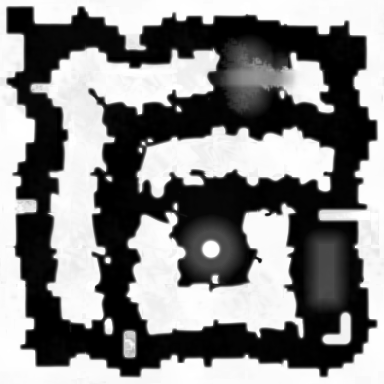
\includegraphics[scale=0.7]{kepek/heightmap.png}
\caption{A magasságmező adatait tartalmazó bitmap}
\label{fig:heightmap}
\end{figure}

\begin{figure}[h]
\centering
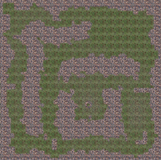
\includegraphics[scale=1.6]{kepek/heightmap_texture.png}
\caption{A magasságmező textúrája}
\label{fig:heightmap_texture}
\end{figure}

\Aref{fig:screenshot} képen pedig a játékban való megjelenés látható. Ez egyben megoldja az ütközéskezelést is, illetve, hogy a túl meredek parton ne lehessen felmenni (lecsúszik róla). A megjelenítendő játéktér részeit egy osztály fogja össze.

\begin{figure}[h]
\centering
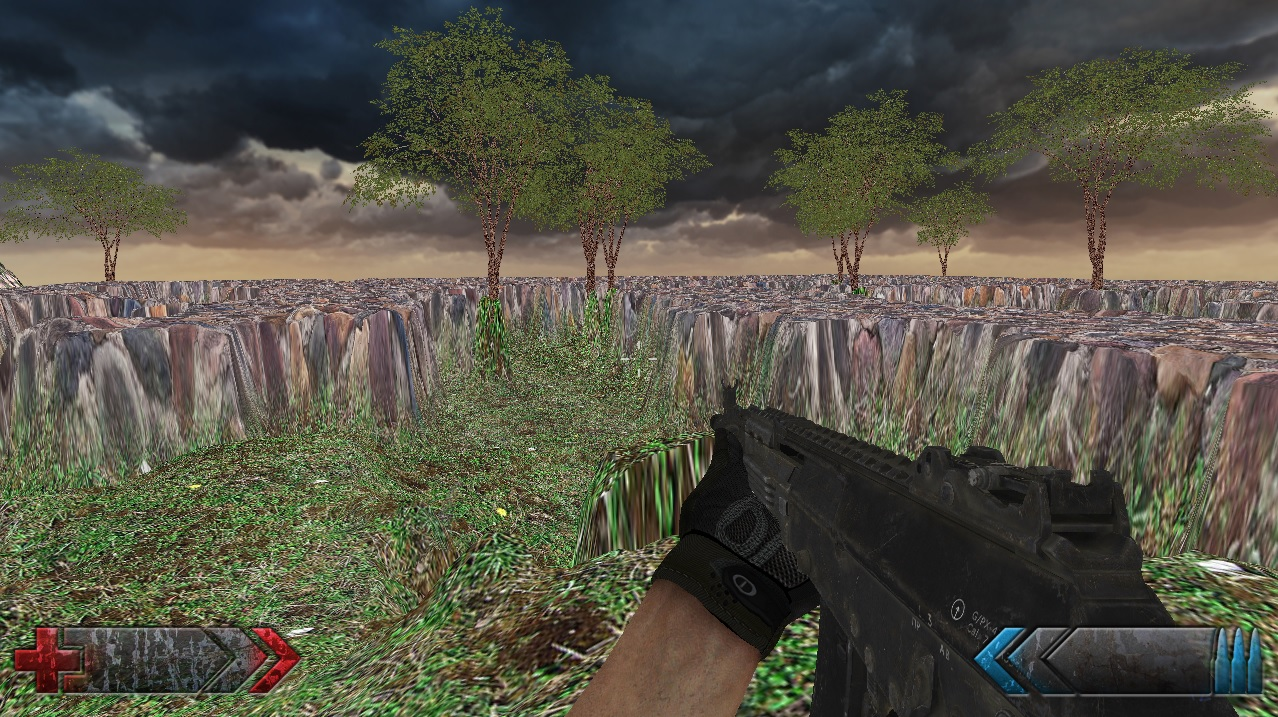
\includegraphics[scale=0.4]{kepek/screenshot.png}
\caption{A megjelenített magasságmező}
\label{fig:screenshot}
\end{figure}

\section{Irányítás, fizika}

A karakterrel előre, hátra, balra illetve jobbra mozogni a WSAD gombokkal, a kamera forgását az egérrel lehet vezérelni. Lehetőség van a SPACE-el ugrani, a CTRL-al guggolni, SHIFT-el gyorsabban menni, illetve a görgő fel/le mozgatásával az egér érzékenységét állítani. A kamera mozgatásához szükséges függvények is, és az állapotok kezeléséhez tartozó változók is külön osztályban vannak. Minden cselekedethez tartozik egy bool (két állapotú) változó. Pl. ha tegyük fel előre megyünk, akkor az ehhez tartozó változó „true (igaz)” értéket vesz fel, amihez különböző eseményeket lehet kötni, mint pl. a kamera előre mozgatását, bizonyos animációk lejátszását.

\section{Hangok}

A hangok megszólaltatáshoz az SDL\_mixer-t veszi segítségül, amiben külön vannak kezelve a háttérzenék, illetve a hangeffektek (lövés, lépés stb.). Háttérzenéhez egyszerre 1 csatorna tartozik, míg hangeffektekhez végtelen. Meg lehet adni, hogy a hang hányszor kerüljön lejátszásra, illetve melyik csatornán. A  NUM +/- gombokkal lehet a hangerőt növelni/csökkenteni, és ezek külön vannak kezelve a menüben, illetve a játékban.

\section{Állapotok}

A játékban jelenleg található egy kezdetleges menü, illetve az ingame rész. Ezek, mint állapotok vannak lekezelve, külön osztályokban megvalósítva. A főmenüért, az ingame objektumokért, magasságmezőért is egy-egy külön osztály felelős. A főmenü \aref{fig:menu} ábrán, a betöltőképernyő pedig \aref{fig:loading} ábrán látható.

\begin{figure}[h]
\centering
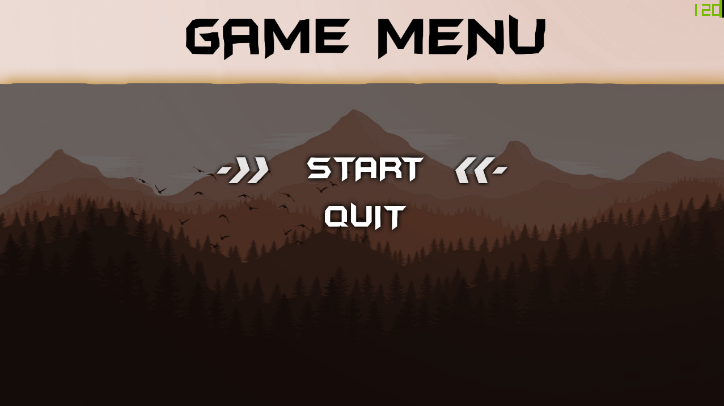
\includegraphics[scale=1.6]{kepek/menu.png}
\caption{A főmenü}
\label{fig:menu}
\end{figure}

\begin{figure}[h]
\centering
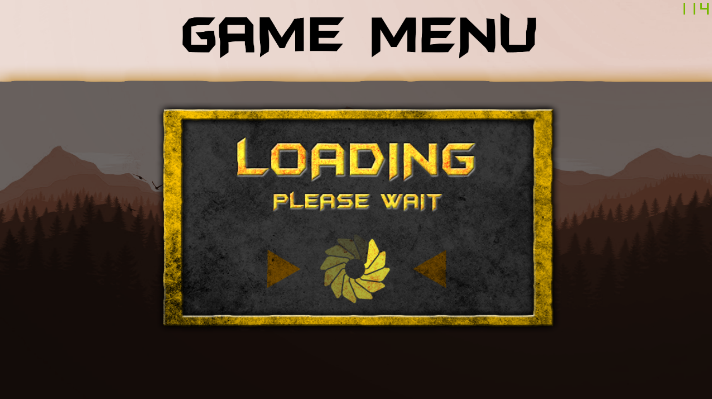
\includegraphics[scale=1.6]{kepek/loading_screen.png}
\caption{Pályabetöltés közben ez látható}
\label{fig:loading}
\end{figure}

\section{Lövés}

A lövés háttérszámításai, matematikai kalkulációk is egy külön komponensnek tekinthetők. Első lépés, hogy ki kell számolni a vektort amerre a játékos néz, minden képkockára. Mivel a világ háromszögekből épül fel, ezért ki kell számolni az egyenes háromszöggel való metszéspontját. De mivel több 100000 háromszögről beszélünk, ez további optimalizálandó problémákat vet fel, amit a későbbiekben fejtek ki.

\section{Mesterséges intelligencia}

Az MI osztálynak elsősorban az a feladata, hogy az ellenfelek egy meghatározott útvonalon mozogjanak, ne menjenek át falakon, menjenek egymásba. A véletlenszerűen lerakott ellenfelet a legközelebbi definiált waypoint-hoz kell irányítani, definiálni kell a célpontot (ami mindig a játékos), és ki kell számítani a pontokon keresztül vezető legrövidebb útvonalat.

\section{A játékindítás folyamata}

Első lépésben a játék létrehozza az SDL ablakot, és konkrétan beállítja annak pozícióját, függőleges és vízszintes felbontását, illetve a flageket, pl. a kurzort, teljes képernyő legyen vagy nem.

A második lépés hogy az előtte létrehozott ablakot beállítja aktívra, és OpenGL megjelenítésre. Létre kell hozni egy érvényes OpenGL  kirajzolás kontextust, hogy inicializáljuk a belépési pontokat. Ez használhatóvá teszi az összes elérhető funkciót, amit az OpenGL magban definiáltak. Ezután betölti a főmenü megjelenítéséhez szükséges modelleket, textúrákat.

Harmadik lépésben aktiválja a hangok megszólaltatásáért felelős komponenst, és betölti az összes hangot, zenét.

A negyedik lépésben pedig aktiválja az eseménykezelő komponenst, ami a felhasználótól érkező interakciókat kezeli, majd meghívja a betöltött modelleket kirajzolásra.

A menübe érkezés után a felhasználónak lehetősége nyílik a játékteret betölteni, vagy kilépni. 

A „Start” gombra kattintás után, betöltődik a magasságmező kezelő komponens, a kamera a kezdőpontra pozícionálódik, elkezdődnek a játékmenethez elengedhetetlen háttérszámítások, és egy új zene lejátszása, betöltődnek a játéktér modelljei, elemei, illetve átvált azok kirajzolására. Hogy a játékos informálva legyen, ez idő alatt megjelenik a betöltőképernyő.

